\documentclass{article}
\usepackage{pgfplots}
\usepgfplotslibrary{colormaps} % Additional color maps
\pgfplotsset{compat=newest} % Use newest version for better compatibility

\begin{document}

\begin{figure}
    \centering
    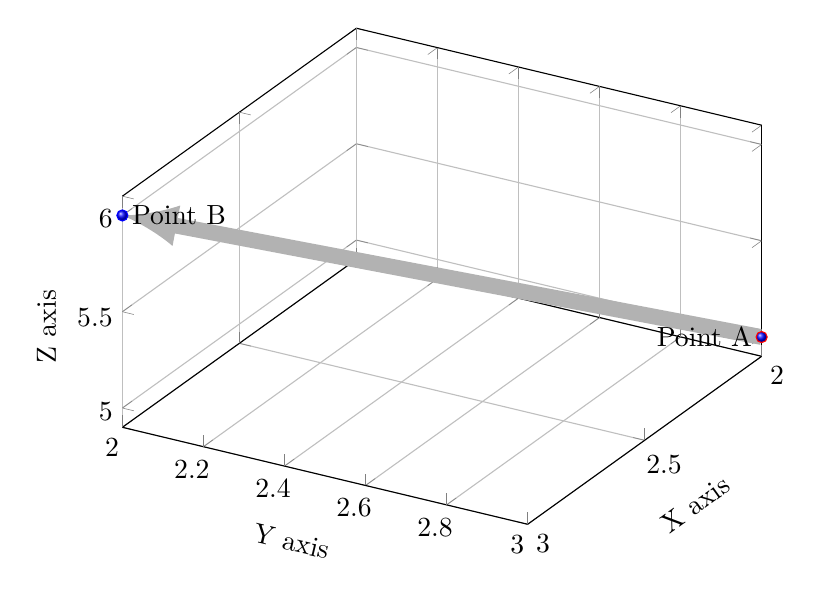
\begin{tikzpicture}
        \begin{axis}[
            xlabel={X axis},
            ylabel={Y axis},
            zlabel={Z axis},
            xlabel style={sloped like x axis}, % Make x label follow the x axis
            ylabel style={sloped like y axis}, % Make y label follow the y axis
            zlabel style={sloped}, % Make z label follow the z axis or make it vertical
            grid=major,
            width=0.8\textwidth,
            height=0.65\textwidth,
            view={120}{40}, % Adjust the view angle for better visualization
        ]
            % Define points
            \addplot3[only marks, color=red, mark=ball] coordinates {(2,3,5)};
            \addplot3[only marks, color=blue, mark=ball] coordinates {(3,2,6)};

            % Draw a "pipe-like" line between points
            \addplot3[
                no marks,
                thick, 
                line width=2mm, % Making the line thicker to simulate a pipe
                color=gray!60, % Choosing a color that stands out with some 3D appearance
                -latex % Adding an arrow tip for direction, optional
            ] coordinates {(2,3,5) (3,2,6)};

            % Optionally, label points
            \node at (axis cs:2,3,5) [left] {Point A};
            \node at (axis cs:3,2,6) [right] {Point B};
        \end{axis}
    \end{tikzpicture}
    \caption{Connecting a point to its nearest neighbor in 3D space with a pipe-like appearance.}
\end{figure}

\end{document}
